% Created 2016-03-09 Wed 21:58
\documentclass{article}
\usepackage[utf8]{inputenc}
\usepackage[T1]{fontenc}
\usepackage{fixltx2e}
\usepackage{graphicx}
\usepackage{grffile}
\usepackage{longtable}
\usepackage{wrapfig}
\usepackage{rotating}
\usepackage[normalem]{ulem}
\usepackage{amsmath}
\usepackage{textcomp}
\usepackage{amssymb}
\usepackage{capt-of}
\usepackage{hyperref}
\author{Taylor Foxhall}
\date{\today}
\title{Simple Line Drawing Algorithms}
\hypersetup{
 pdfauthor={Taylor Foxhall},
 pdftitle={Simple Line Drawing Algorithms},
 pdfkeywords={},
 pdfsubject={},
 pdfcreator={Emacs 24.5.1 (Org mode 8.3.3)}, 
 pdflang={English}}
\begin{document}

\maketitle

\section{Introduction}
\label{sec:orgheadline1}
We'll be examining the Sutherland-Hodgman clipping algorithm, floodfilling, and demonstrating window to viewport mapping.
\section{Clipping}
\label{sec:orgheadline4}
\subsection{Idea}
\label{sec:orgheadline2}
Sutherland-Hodgman clips non-concave polygons with a rectangular clipping window, although in practice this implementation
shouldn't be limited to just rectangular clipping windows. The algorithm will follow the edges of a provided clipping window
and observe if the edges of the polygon being clipped are outside, inside, or intersecting the edge of the clipping window.
It then eliminates vertices or adds new intersections and passes that set onto the next edge, which repeats until all edges
are visited.
\subsection{Code Exposé}
\label{sec:orgheadline3}
\begin{verbatim}
void clip(const std::list<Point2d>& clip_window) {
  std::list<Point2d> output_verts;

  for (auto& pic: painter.get_drawings()) {
    output_verts = pic->get_points();

    for (auto it = clip_window.cbegin(); it != clip_window.cend();) {
      std::pair<Point2d, Point2d> clip_edge;
      if (it == --clip_window.cend()) {
        clip_edge = std::make_pair(*it, *clip_window.cbegin());
        it++;
      } else {
        clip_edge = std::make_pair(*it, *(++it));
      }
      auto input_verts = output_verts;
      output_verts.clear();
      auto last = input_verts.back();
      // Clipping assumes vertices are drawn counterclockwise
      for (auto& p: input_verts) {
        if (inside_boundary(clip_edge.first, clip_edge.second, p)) {
          if (!inside_boundary(clip_edge.first, clip_edge.second, last)) {
            // outside -> inside
            output_verts.push_back(intersect(std::make_pair(p, last), clip_edge));
          }
          // inside -> inside or outside -> inside
          output_verts.push_back(p);
        } else if (inside_boundary(clip_edge.first, clip_edge.second, last)) {
          // inside -> outside
          output_verts.push_back(intersect(std::make_pair(p,last), clip_edge));
        }
        last = p;
      }
    }
    viewport_painter.add_drawing(output_verts);
  }
}
\end{verbatim}
\section{Region filling}
\label{sec:orgheadline7}
\subsection{Idea}
\label{sec:orgheadline5}
Floodfilling is well established and rather simple. The algorithm simply picks a starting point (in this case provided by
where the user's mouse is when the 'f' key is pressed) and expands out in a four-connected fashion using breadth-first search.
The pixels visited are stored in an unordered set, and then drawn in red when they are visited.
\subsection{Code Exposé}
\label{sec:orgheadline6}
\begin{verbatim}
unsigned char pixel[4], base_color[4];
int width = glutGet(GLUT_WINDOW_WIDTH);
int height = glutGet(GLUT_WINDOW_HEIGHT);
std::queue<Point2d> to_visit;
std::unordered_set<Point2d, Point2dHash> seen;
const std::list<Point2d> neighbors {std::make_pair(1,0), std::make_pair(0,1), std::make_pair(-1,0), std::make_pair(0,-1)};
glReadPixels(start.first, start.second, 1, 1, GL_RGBA, GL_UNSIGNED_BYTE, &base_color);

to_visit.push(start);
while (!to_visit.empty()) {
  auto pt = to_visit.front();
  to_visit.pop();
  _verts.push_back(pt);

  // Visit neighbors
  for (auto& n: neighbors) {
    auto n_x = pt.first + n.first, n_y = pt.second + n.second;
    auto np = std::make_pair(n_x, n_y);
    if (seen.count(np) == 0 && !(n_x < 0 || n_x > width || n_y < 0 || n_y > height)) {
      glReadPixels(n_x, n_y, 1, 1, GL_RGBA, GL_UNSIGNED_BYTE, &pixel);
      if (pixel[0] == base_color[0] && pixel[1] == base_color[1] && pixel[2] == base_color[2] && pixel[3] == base_color[3]) {
        seen.insert(np);
        to_visit.push(np);
      }
    }
  }
}
\end{verbatim}
\section{Viewport Mapping}
\label{sec:orgheadline10}
\subsection{Idea}
\label{sec:orgheadline8}
The viewport mapping algorithm is rather basic: simply translate the vertices you want to map by (-window.xmin, -window.ymin),
scale down by the window dimensions, then back up with the viewport dimensions, then translate by (viewport.xmin, viewport.ymin).
With this, changing the viewport and window size gives us zooming and scaling for free, and panning is obtained simply by
remembering the original polygon that was clipped.
\subsection{Code Exposé}
\label{sec:orgheadline9}
\begin{verbatim}
void map_viewport() {
  // Draw painter's drawings that lie in the clipping window
  viewport_painter.delete_drawings();
  std::list<Point2d> bounds{
    std::make_pair(clip_window.x, clip_window.y),
      std::make_pair(clip_window.x+clip_window.w, clip_window.y),
      std::make_pair(clip_window.x+clip_window.w, clip_window.y+clip_window.h),
      std::make_pair(clip_window.x, clip_window.y+clip_window.h)
      };
  clip(bounds);
  for (auto& pic: viewport_painter.get_drawings()) {
    for (auto& pt: pic->get_points()) {
      if (clip_window.contains(pt)) {
        Point2d t1 = std::make_pair(pt.first-clip_window.x, pt.second-clip_window.y);
        Point2d t2 = std::make_pair(static_cast<int>(t1.first * (static_cast<double>(viewport.w)/clip_window.w)),
                                    static_cast<int>(t1.second * (static_cast<double>(viewport.h)/clip_window.h)));
        Point2d t3 = std::make_pair(t2.first+viewport.x, t2.second+viewport.y);

        if (!viewport_painter.is_painting()) {
          viewport_painter.start_drawing(t3);
        } else {
          viewport_painter.add_point(t3);
        }
      }
    }
    if (viewport_painter.is_painting()) {
      viewport_painter.stop_drawing();
    }
  }
}
\end{verbatim}
\section{Demos}
\label{sec:orgheadline11}
\begin{figure}[htb]
\centering
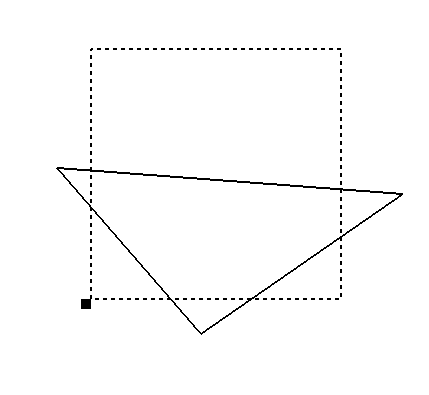
\includegraphics[width=.9\linewidth]{./img/unclipped.png}
\caption{A triangle lying insde a clipping window}
\end{figure}
\begin{figure}[htb]
\centering
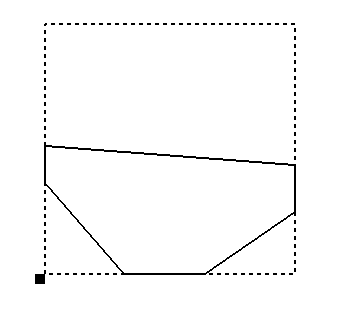
\includegraphics[width=.9\linewidth]{./img/clipped.png}
\caption{The triangle is clipped}
\end{figure}
\begin{figure}[htb]
\centering
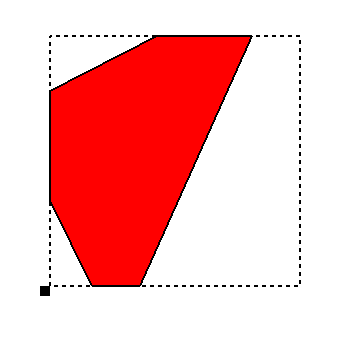
\includegraphics[width=.9\linewidth]{./img/floodfill.png}
\caption{The result of floodfill on a clipped triangle}
\end{figure}
\begin{figure}[htb]
\centering
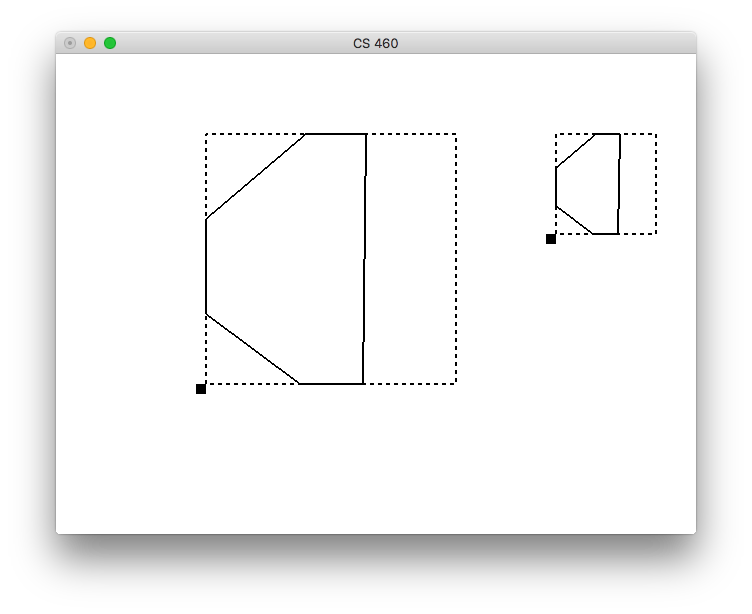
\includegraphics[width=.9\linewidth]{./img/viewport.png}
\caption{Displaying a clipped polygon in a viewport}
\end{figure}
\begin{figure}[htb]
\centering
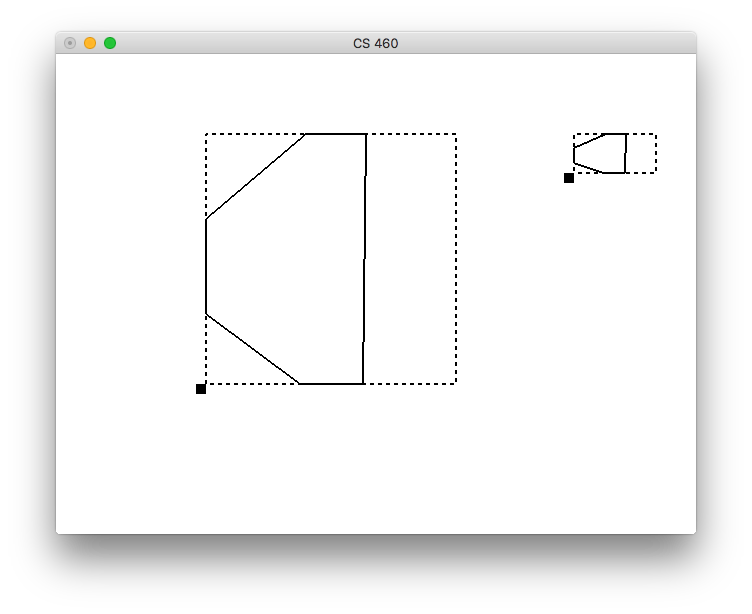
\includegraphics[width=.9\linewidth]{./img/scaled_in.png}
\caption{Scaled displays of the polygon}
\end{figure}
\begin{figure}[htb]
\centering
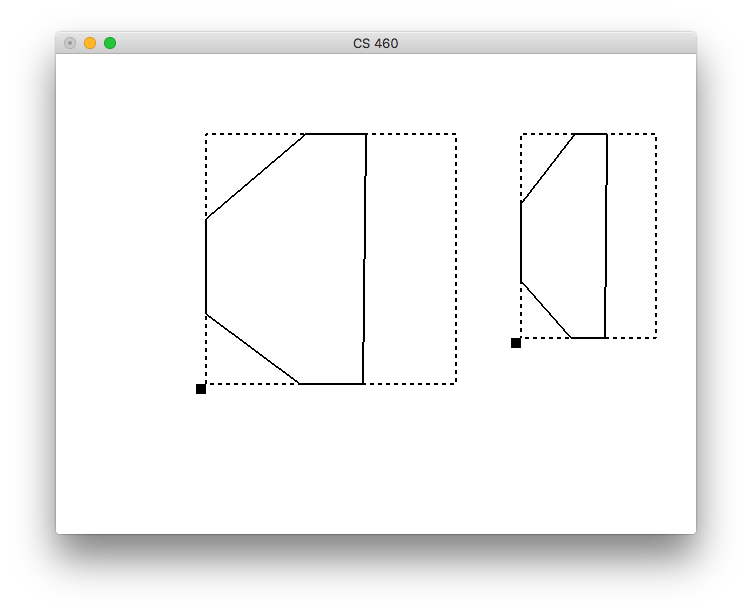
\includegraphics[width=.9\linewidth]{./img/scaled_out.png}
\caption{Scaled displays of the polygon}
\end{figure}
\begin{figure}[htb]
\centering
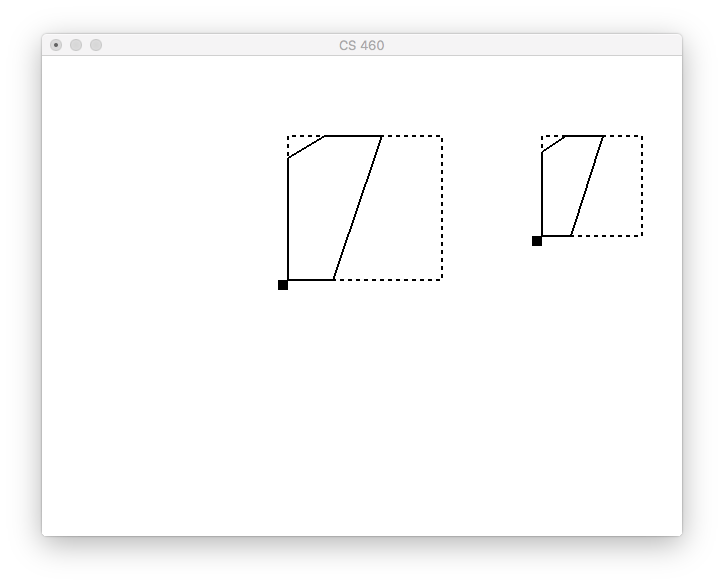
\includegraphics[width=.9\linewidth]{./img/zoom_in.png}
\caption{Zoomed displays of the polygon}
\end{figure}
\begin{figure}[htb]
\centering
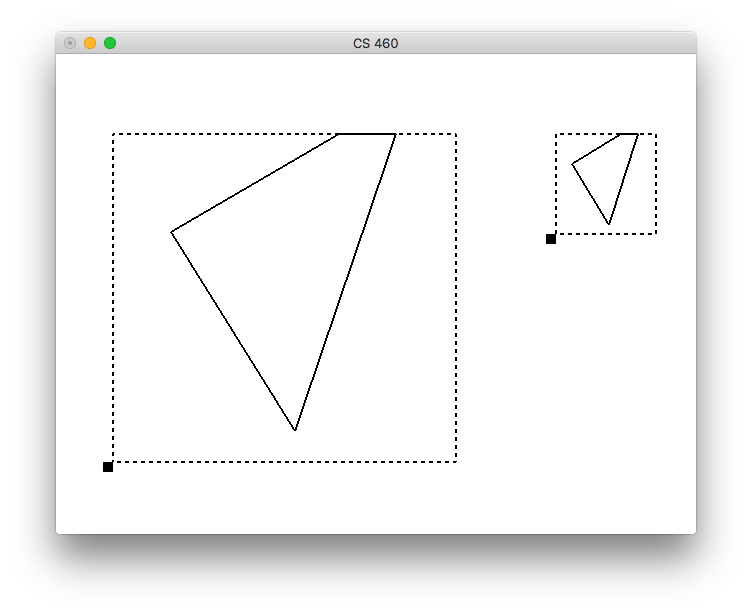
\includegraphics[width=.9\linewidth]{./img/zoom_out.png}
\caption{Zoomed displays of the polygon}
\end{figure}
\begin{figure}[htb]
\centering
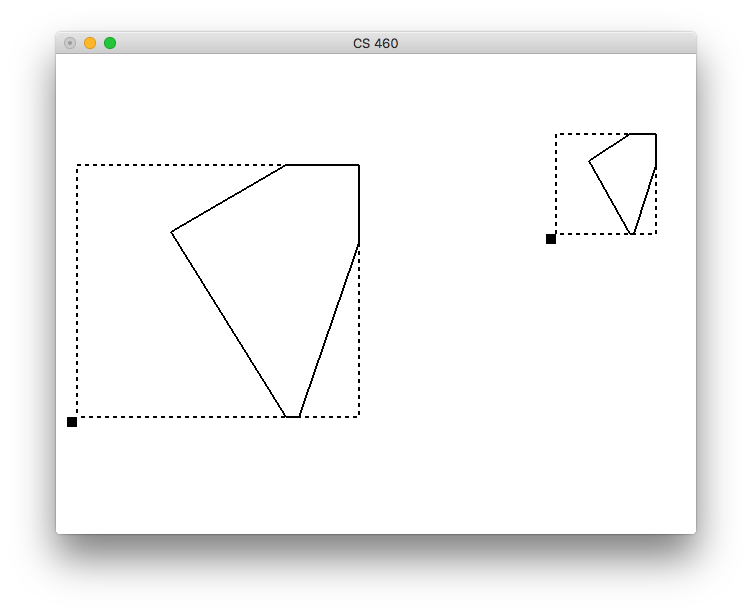
\includegraphics[width=.9\linewidth]{./img/pan.png}
\caption{Panning a window}
\end{figure}
\end{document}